\chapter{Methodology}
\label{chap:methodology}
\begingroup
\justifying
\setlength{\parindent}{2em}
\setlength{\parskip}{0.55\baselineskip}

\section{Experimental logic}

The methodology links the three research questions to observable evidence. RQ1 requires generated plans that can be simulated and navigated, plus qualitative and performance evidence that dense scenes remain usable. RQ2 requires a documented path from task specification to successful demonstrations and a stable policy interface. RQ3 requires controlled splits, repeated trials and failure labels. No single number answers all three.

The experimental unit is a policy episode in a generated store environment. An episode is defined by a task, named target, fixture context, environment seed and evaluation scenario. The policy receives only language, RGB observations and proprioception through its adapter. Ground-truth object and fixture state remain inside the simulator for resetting and success evaluation. Demonstration generation is allowed privileged state because its purpose is to create supervision, not to serve as a baseline policy.

Three principles reduce ambiguity. All four policies train on demonstrations produced by the same system. Evaluation uses the same task predicates and scenario definitions. Composite tasks use the same oracle decomposition for every model. Training recipes differ where model implementations require it, and this is reported rather than disguised as a fully controlled architecture ablation.

\section{Scene synthesis procedure}

For each store, the pipeline samples or loads the store dimensions, fixed fixtures and generation parameters. Collision-free random placement establishes boundary conditions, after which the tensor field of Equations~\ref{eq:basis-tensor} and~\ref{eq:tensor-field} is queried at each candidate position as the sweep advances. The local principal direction admits or rejects an axis-aligned shelf rather than setting its angle, as the system chapter describes; admitted candidates are then tested against occupied polygons and passage margins. Horizontal and vertical sweeps continue until the plan is filled or no valid candidates remain.

The procedure makes two types of failure explicit. A candidate-level failure is simply rejected; generation continues. A scene-level failure occurs when configured constraints cannot be satisfied, in which case the seed is not used as a valid evaluation scene. This distinction prevents infeasible geometry from being mistaken for a policy failure.

Product arrangement is conditioned on the accepted fixtures. Support surfaces are detected, product groups are selected and occupancy grids are constructed. Small pose perturbations diversify appearances while maintaining stable contacts. A depletion mechanism for shelf occupancy was designed but was not used to generate any scene in this study. Textures for the walls, floor, ceiling and doors are drawn from independent pools. For the reported policy experiment, fully stocked shelves are retained so the principal shifts are layout, texture and task--item pairing rather than depletion.

Scene quality is evaluated by construction checks and inspection. Collision rejection and passage constraints provide geometric validity. Rendered examples offer an author-inspection sanity check: the tensor-guided plans appear store-like rather than randomly scattered. Simulation performance tests compare original and simplified product geometry across increasing shelf counts. These checks do not prove realism in a user-study sense; they establish that generated scenes meet the project's operational requirements.

\section{Trajectory sampling procedure}

Each atomic task is decomposed into stages such as base approach, pre-grasp, grasp, lift, transport, pre-place and release. Task-specific code samples anchor poses around the true target state. Random perturbations of anchors and initial robot pose introduce demonstration variety without removing feasibility.

\ref{fig:anchor-sequence} sets out the loop. Planning proceeds segment by segment. When the base remains fixed, the sampler attempts a screw-motion trajectory. The path is executed only after collision validation. The implementation allows a second screw attempt before falling back to RRT-Connect, which searches explicitly through configuration space. Segments requiring base movement call a task-specific approach planner. The complete candidate trajectory is run in simulation. If planning fails, collision invalidates the motion or the task predicate is not satisfied, the episode is discarded and collection restarts from a reset environment.

\begin{figure}[H]
    \centering
    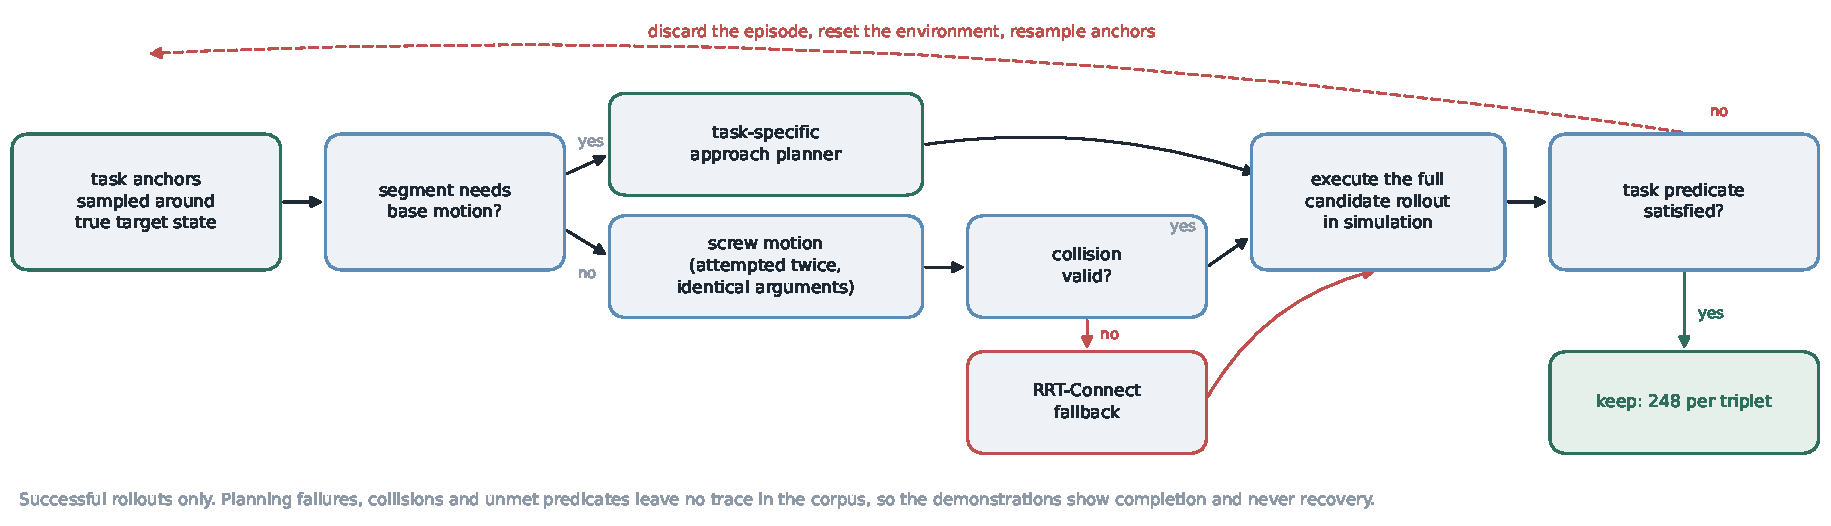
\includegraphics[width=\textwidth]{assets/figures/retail-vla-benchmark/collector_pipeline.pdf}
    \caption{The demonstration collector. Anchors are sampled using privileged object state; each segment is planned by screw motion where the base is fixed and by a task-specific approach planner where it is not; RRT-Connect catches segments that fail collision validation. Only complete rollouts that satisfy the task predicate enter the corpus, and everything else returns to the top of the loop. The two screw attempts are made with identical arguments, so for a deterministic solver the second cannot succeed where the first failed.}
    \label{fig:anchor-sequence}
\end{figure}

Retaining only successful executions produces clean imitation targets and a simple data contract. It also creates selection bias. Demonstrations concentrate on trajectories the planner can solve and omit failed approaches, recovery actions and ambiguous grasps. A learned policy may therefore imitate nominal behaviour without learning how to return to it after a small error. This limitation is revisited when interpreting grasp and pre-grasp failures.

Collected episodes are stored in HDF5 with accompanying metadata, and conversion to other training formats is handled outside the core benchmark. Storage requirements depend on the image encoding, metadata retained and dataset revision; the archived study materials do not support a sufficiently stable size estimate to report one here.

\section{Training protocol}
\label{sec:training}

Octo, SmolVLA, $\pi_0$ and $\pi_{0.5}$ were fine-tuned on a single NVIDIA RTX 4090 using the implementations and configurations recorded in this study. All four use batch size 8, and every run stopped when its preset step counter expired rather than when its loss settled. The comparison that follows is therefore between four fixed-step study configurations, none of which was verified to have converged.

Three of the four use low-rank adaptation. SmolVLA is adapted for 100,000 steps at batch size 8 with rank 64 and $\alpha=64$ on the language expert's query and value projections together with the state and action projections, at a learning rate of $1\times10^{-3}$ decaying by cosine to $1\times10^{-4}$, taking approximately two hours. $\pi_0$ and $\pi_{0.5}$ are adapted for 30,000 steps at batch size 8 with rank 16 on the vision--language backbone and rank 32 on the action expert, applied to the Gemma attention and feed-forward blocks of both, taking approximately two and a half hours each; $\pi_0$ uses AdamW at $2.5\times10^{-5}$ with 1,000 warmup steps and cosine decay to $2.5\times10^{-6}$, while $\pi_{0.5}$ uses $5\times10^{-5}$ with 10,000 warmup steps held constant thereafter, and EMA is disabled for both. Octo is the exception in the recorded study configuration: it is fully fine-tuned for 100,000 steps at batch size 8, also in about two hours, retaining two history observations and a continuous action head.

All four keep an action horizon of 50. Durations are descriptive records from this study, not normalised efficiency comparisons. Step budgets were selected separately for the four implementations under the available hardware rather than matched across models, and no controlled experiment establishes that any one budget was sufficient.

The policies are trained only on atomic tasks. No composite demonstration is used. At evaluation, the oracle issues the next atomic language instruction after the current predicate succeeds. Consequently, any non-zero composite score would demonstrate that an atomic policy can maintain competence across state changes caused by earlier actions. Zero composite performance does not, by itself, reveal whether the problem is long-horizon memory, compounding atomic error or the changed post-action observation distribution.

\section{Evaluation scenarios}
\label{sec:scenarios}

The generator exposes six variation axes: initial robot position, texture, store layout, shelf arrangement, products withheld from a given task and products withheld entirely. The main study combines them into three cumulative conditions, each named for the variable it introduces rather than by an abbreviation.

\textbf{Pose} randomises the robot's start within a task-relevant region and holds everything else at its training value. It tests local robustness to where the robot happens to be standing.

\textbf{Layout} adds new store plans and new floor, wall and ceiling materials. The task and its training products stay familiar; the geometry around them and the visual context do not.

\textbf{Pairing} additionally names a target that was never demonstrated on the evaluated task, though it was demonstrated on another. The shift is compositional rather than perceptual: the product is familiar, the skill is familiar, and only the combination is new. It is therefore a weaker test than one involving a product never encountered anywhere. Section~\ref{sec:verification} explains how the products' presence in the training scenes further limits the claim.

A fourth condition, \textbf{Seeds}, appears only in the per-item tables of Appendix~\ref{app:training-results}. It reruns the stored configurations used to collect the demonstrations and changes nothing at all, which is what makes it useful: it separates imitation of the training distribution from any transfer beyond it.

The software supports unseen shelf arrangements and completely unseen items, yet the headline experiment excludes them. This is a methodological choice based on observed model weakness in simpler settings. It avoids spending most of the evaluation budget on uniformly zero conditions, although it also means the benchmark's most difficult generation capabilities are not validated by the reported baseline table.

Two caveats attach to the definitions above, and both were found after the runs were complete. Layout is realised as described for the three pick-and-place families, whose evaluation scenes come from a seed family disjoint from training. It is not realised as described for the four door tasks, which are evaluated on their own training scenes with only the episode and initial-pose seeds changed, so for those tasks Layout varies texture and starting pose but not geometry. Pairing is realised as described in the sense that its target products were never demonstrated on the evaluated task, but those products stand on the shelves of the training scenes throughout adaptation, which is exactly why the condition is named for the pairing and not for the product. A separate code reading first raised both issues; the author then reproduced them before they were retained. Section~\ref{sec:verification} works through their effect on interpretation.

For each task--item--fixture triplet, 100 trials estimate success. Task-level values in the main table pool the applicable equal-sized triplets. Under Pose and Layout, Basket and Board each pool three triplets, while Floor, Open and Close pool two. Under Pairing, each applicable pick-and-place task pools two held-out product triplets. Door tasks have no meaningful Pairing condition because their instructions never name a product, so those cells are marked not applicable rather than zero. This distinction is essential: zero denotes attempted trials with no successes; not applicable denotes an undefined combination.

\section{Success and side-effect checks}

The task predicate combines goal state, collateral state and robot stability. For a target item $o^*$ and destination region $G$, a simplified pick-and-place predicate can be written as
\begin{equation}
  y=\mathbb{I}[o^*\in G]\,\mathbb{I}[\text{robot static}]\,
  \prod_{o\in\mathcal{N}(o^*)}\mathbb{I}[\Delta(o)\leq\epsilon],
  \label{eq:strict-success}
\end{equation}
where $\Delta(o)$ is non-target displacement, $\epsilon$ is the implementation tolerance and $\mathcal{N}(o^*)$ is the set of non-target products the check actually visits. Both of the last two deserve to be stated rather than left as symbols. The tolerance is 0.1 in position, applied per component together with an equal tolerance on the quaternion, so a neighbour has to shift by roughly ten centimetres before the episode is invalidated. And $\mathcal{N}(o^*)$ is not the whole scene. For the basket task, the evaluator restricts this check to products on the target fixture, which means stock knocked from a neighbouring shelf during the approach goes uncounted. The other pick-and-place tasks range over the scene.

$G$ is likewise more forgiving than the prose suggests. Containment is an axis-aligned box test applied per coordinate rather than a Euclidean distance, so the threshold of 0.2 acts as a half-extent and the accepted region is a cube 0.4~metres on a side; one product uses 0.25. For basket picking that cube is anchored to the robot's own base rather than to a fixed point in the store. Board transfer is tighter, roughly ten centimetres horizontally, with its goal defined as the item's initial position raised by the 0.397~metre clearance between boards. A successful placement is still rejected if surrounding stock moved or the robot has not settled; the thresholds simply describe a looser test than the system chapter originally implied.

Door predicates instead inspect articulation state and stability, which avoids asking a human observer whether a door ``looks open'' but makes the result sensitive to a threshold choice. The showcase requires its named door joint to reach $1.57$~rad within $\pm 0.2$~rad for opening or zero within the same band for closing. The refrigerated fixture is different on both counts: its cover joint has to reach $0.624$~rad, a little under thirty-six degrees, and the tolerance is $\pm 0.1$~rad. Opening a fridge in this benchmark therefore means swinging a door through about two fifths of the arc a showcase door travels, judged twice as strictly. Neither constant is optimal in any principled sense. They are reported so that the numbers in the results chapter can be audited against them.

Mean success is reported as a percentage. Where two conditions can be paired at task level, absolute degradation is
\begin{equation}
  \Delta S_{m,t}=S_{m,t,\mathrm{Pose}}-S_{m,t,\mathrm{Layout}}.
  \label{eq:degradation}
\end{equation}
Absolute percentage-point loss is preferred to a relative percentage for near-zero baselines, where ratios become unstable or undefined.

\section{Failure annotation}

Failed episodes are sampled for qualitative annotation. For each model, approximately ten unsuccessful episodes are drawn from each applicable task--item--fixture combination across Seeds, Pose, Layout and Pairing. The study record reports 2,906 labelled failures. That total does not follow from the procedure just described: the four models and the strata they span imply roughly a hundred and seventy combinations, and 2,906 labels across them averages about seventeen per combination rather than ten. Neither the realised sampling frame nor the episode identifiers were retained with the reported aggregates, so the difference cannot be explained, and neither this total nor the percentages derived from it can be independently re-aggregated from the archived materials. The figure is reported as the study recorded it, and the failure percentages should be read as descriptive of that record rather than as an auditable sample. The annotator records the earliest primary failure visible in the pipeline.

The categories are ordered: \emph{task}, \emph{target}, \emph{move}, \emph{pregrasp}, \emph{grasp}, \emph{drop}, \emph{displace}, \emph{preplace}, \emph{place-coord}, \emph{place} and \emph{partial}. ``Task'' means the behaviour corresponds to another requested operation. ``Target'' means the robot acts on the wrong product. ``Move'' and ``pregrasp'' separate mobile-base approach from local alignment. ``Grasp'' denotes failure to secure the product or handle despite reaching it. The next two categories capture loss of a grasp and disturbance of other products. Placement is divided into approach, coordinate selection and release. ``Partial'' is reserved for incomplete door articulation.

This coding scheme is diagnostic but not perfectly objective. Only unsuccessful episodes are annotated. Labels are assigned manually, and the earliest-failure rule suppresses later consequences. No inter-rater agreement is reported. The distributions should therefore be used to identify large, repeated patterns---for example, grasp accounting for 40\% of $\pi_{0.5}$ failures---rather than to distinguish close percentages as if they were precise sensor measurements.

\section{Validity considerations}
\label{sec:validity}

The controlled parts of the experiment are clear. All four policies receive demonstrations from the same collector, scenes from the same generator and judgements from the same task predicates. The comparison ceases to be matched at adaptation. Each model stops at a preset step count, three use low-rank updates while Octo is fully fine-tuned, and no run is selected by validation performance. Model size, pretraining, optimisation and distance from convergence therefore move together. The table compares four complete study pipelines, not four architectures.

The executed protocol also differs from the written design in several places. A separate reading of the code first raised these discrepancies; the author then reproduced each retained item and classified it as more permissive, more restrictive, or descriptive only. Section~\ref{sec:verification} reports the resulting audit. Unresolved provenance is labelled as such, rather than converted into a directional claim.

Construct validity is narrower than the scale of the generated stores might suggest. The tasks cover cluttered picking, shelf transfer, door articulation and local base positioning. They do not cover store-scale navigation. Every episode begins 1.4~metres from the correct fixture and facing it, with modest translation and yaw perturbations applied on top. The aisles constrain scene geometry and camera context; policies never have to traverse them. Barcode scanning, deformable packaging, people, moving obstacles and damage detection are absent as well.

Control is constrained in two further ways. The policy receives a new observation only after a fifty-action chunk has executed, so it cannot react to contact or pose changes during that interval. Torso lift and head pan are fixed at zero. Conclusions about grasp precision or whole-body reach are conditional on both choices.

External validity remains limited to simulation. The study says nothing direct about sensing noise, friction, compliance, calibration or deformable packaging in a physical store. Statistically, its hundred trials per triplet yield useful point estimates, but the retained task-level aggregates omit episode pairing and layout grouping. They cannot support design-aware condition contrasts. Episode-level outcomes would have allowed paired comparisons, seed-level bootstrap intervals or a mixed-effects treatment of item and layout variation; those records were not preserved in the archived bundle.

\section{Protocol traceability and quality control}
\label{sec:traceability}

Traceability begins with a chain from each reported cell to the checkpoint, code version, scene configuration, prompt and terminal decision that produced it. Seeds alone are insufficient. Layout, arrangement and initial-pose identifiers should be frozen before evaluation, while episode-level outcomes should remain available after aggregation. The present dissertation preserves the reported values and their transformation rules, but not that complete chain.

The same discipline applies at the interface. Camera shape and colour order, proprioceptive fields, action scaling and the ordering of all thirteen commands require explicit checks. Task predicates need positive and negative unit tests at their thresholds. Checkpoint selection should use a validation split, followed by one evaluation on frozen test seeds; repeated attempts, if unavoidable, should be retained.

Failure labels need synchronised views, a written codebook and a second annotator on a stratified subset. Figures and tables should then be generated from the same machine-readable episode records. These steps would turn the next run of this dissertation project from a documented aggregate study into one whose results can be re-analysed without reconstructing lost experimental context.

\endgroup
